\documentclass[12pt]{report} % 10, 11 (default) or 12
\usepackage[dutch]{babel}
% Instead of using \\ (or \newline/\vspace) to simulate paragraph breaks, or to increase inter-paragraph spacing,
% the recommended solution for setting spacing between paragraphs is to load the parskip package:
% put \usepackage{parskip} in your document’s preamble.
% https://ctan.org/pkg/parskip
\usepackage{lipsum}
\usepackage{graphicx}
\graphicspath{ {images/} }

\usepackage{array}
\usepackage{colortbl}
\usepackage[utf8]{inputenc}

\setlength{\arrayrulewidth}{1mm}
\setlength{\tabcolsep}{18pt}
\renewcommand{\arraystretch}{1.5}

\begin{document}
\tableofcontents

%%%
%%%
%%%
\chapter{Inleiding}
Wij danken U voor de aanschaf van het marIntegraal administratiepakket en zijn ervan
overtuigd dat alle mogelijkheden zullen voldoen aan uw huidige bedrijfsbehoeften.

\section{1985 $=>$ CP/M - MSDOS}
marIntegraal werd december 1985 door Vsoft voor het eerst op de markt gebracht voor
AMSTRAD JOYCE PCW tekstverwerkingssysteem, welke eveneens kon omgetoverd worden tot
volwaardig CP/M PLUS computersysteem mét Mallard Basic als gratis programmeertaal.

marIntegraal is in eerste versie geschreven met deze Mallard BASIC (supersnelle
MS BASIC compatibele programmeertaal mét ingebouwd een uitzonderlijk degelijk en snel
multi-user BTRIEVE systeem voor database beheer), op dat ogenblik 1985-1986 meest
interessant platform voor boekhoudsoftware op microcomputer!

In 1986 lanceert weerom AMSTRAD de eerste low-cost PC-compatibele mét terug standaard
Mallard BASIC beschikbaar. Vsoft onderschrijft met Locomotive Software een
licentiecontract om marIntegraal te kunnen verdelen op alle PC-compatibelen.

\section{1995 $=>$ WINDOWS}
Voor marIntegraal NT onder Windows wordt bij gebrek aan enige licentiemogelijkheid
met Locomotive Software voor Mallard Basic tot einde 1998 gebruik gemaakt van
NOVELL's BTRIEVE met record-pér-record beveiliging, welke het onmiddellijk toepasbaar
maakt als 'veilig' systeem in alle netwerken voor WINDOWS.

Vanaf 1999 zal BTRIEVE (afstoot door NOVELL) vervangen worden door MS-ACCESS,
de ‘MS-JET‘MS-JET’ krachtbron van Microsoft. De gebruiker zelf zal voor deze overstap
geen andere werkwijze dienen aan te leren.

Tot op heden draait de PC versie van marIntegraal nog steeds op de MS-JET krachtbron
en kan de gebruiker via de MarioApp de data synchroniseren met naar eigen keuze
SQL Server, MySQL enz.

\section{M.A.R.}
De afkorting M.A.R. staat voor "Minimumindeling van het Algemeen Rekeningstelsel"
(van 1976-1982 gekend als M.G.R.-stelsel : Minimum genormaliseerd rekeningstelsel).

Deze voorletters zijn speciaal opgenomen om de hoofdtaak van het pakket te
beklemtonen: namelijk het voeren van een gereglementeerde Belgische boekhouding.

\subsection{Belgisch}
Het pakket wordt aangeboden als een der weinige dat van de eerste tot de laatste
letter geschreven is met de Belgische Wetgeving als beginsel en leidraad.
Noch vertaling, noch aanpassing van een bestaand buitenlands programma!

Het nauwgezet volgen van de Belgische wetgeving, zorgt voor een degelijke basis
en opvolging van nieuwe normen die een Europese Unie met zich mee brengt.

\subsection{Administratie pakket}
Naast de klassieke boekhoudkundige verrichtingen (aankoopboek, verkoopboek,
10 financiële boeken, financieel kruisposten boek, proef- en saldibalans,
investeringsboek, algemeen journaal, historieken, jaarverslag e.a.), verzorgde het
pakket vanaf 1988 eveneens diverse randadministraties zoals opvolging klanten en
leveranciers, mailing en briefwisseling, stockbeheer, prijsberekening, communicatie
met de buitenwereld via bestandsoverdracht naar STAAT (N.B.B., BTW),
BANK (overschrijvingen) en LEVERANCIERS.

\section{Set-up Bedrijf}
Opbouw factuur lay-out in 4 talen, hoofdrekeningen voor automatische boekingen,
afbakening boekjaar, periodieke afsluitingen, installatie tellers facturen, offertes,
bestelbons, leveringsbons, financiële documenten, bladzijden journalen, teksten
etiket kassaverkoop, maatstaven producten (4 talen) e.d.

\section{Boekjaren per bedrijf}
2 actieve en 10 opvraagbare boekjaren.
Per bedrijf kan de gebruiker 2 boekjaren 100\% op een wettelijke wijze bewerken.

Vooral voor boekhoudkantoren, alsook voor snelle jaarovergang is dit een 'must'.
10 boekjaren pér bedrijf blijven controleerbaar en alle documenten, balansen en
lijsten heruitdrukbaar !

marIntegraal maakt het vanaf 2003 mogelijk om boekhoudstukken gestructureerd te
versturen via het internet. Hetzij naar BTW administraties, N.B.B., Uzelf vanuit
de webwinkel en/of andere online toepassingen voor uw cliënteel.

Van essentieel belang is dat u via marIntegraal NET vooral uw btwadministratie,
intrastat, aankoop- en verkooplogica alsook inkomende en uitgaande betalingen 100\%
kunt gaan automatiseren..

\section{Systeemvereisten}
Het pakket is in huidige PC versie beschikbaar als 32-bits applicatie, draaiende
onder Windows 2000 of hoger.

Verder is er een internet verbinding wenselijk voor de
periodieke download van de updates.

\section{Contacteer ons}
Stel uw vragen via het contactformulier op https://www.vsoft.be

\chapter{Simple booking}

\lipsum

%%%
%%%
%%%
\chapter{Tabellen}

\section{Rekening stelsel/Ledger Account}

Table \ref{table:marintegraal_ledgeraccount_fields} Fields definition of ledgeraccount table.
\begin{center}
    \begin{table}[!ht]
    \centering
    \begin{tabular}{ l m{0.5cm}  m{10em} r }
        \noalign{\hrule height 1pt}
        \cellcolor[gray]{0.9} \textbf{N} &
        \cellcolor[gray]{0.9} \textbf{T} &
        \cellcolor[gray]{0.9} \textbf{Info} &        
        \cellcolor[gray]{0.9} \textbf{L} \\
        \noalign{\hrule height 1pt}
        Id & S* & Account number MAR & 7\\
        V020 & S & Account naming & 40\\
        Dece022 & M & Booking year &\\
        Dece023 & M & Booking year-1 &\\
        Dece024 & M & Booking year-2 &\\
        Dece025 & M & Booking year-3 &\\
        Dece026 & M & Booking year-4 &\\
        Dece027 & M & Booking year-5 &\\
        Dece028 & M & Booking year-6 &\\
        Dece029 & M & Booking year-7 &\\
        Dece030 & M & Booking year-8 &\\
        Dece031 & M & Booking year-9 &\\
        Dece999 & M & Dummy for test &\\
        V021 & S & Distribution key & 50\\
        V032 & S & Budget Flag & 1\\
        V216 & S & Forfait cumulator &
    \end{tabular}
    \caption{Ledgeraccount fields definition}
    \label{table:marintegraal_ledgeraccount_fields}
    \end{table}
\end{center}

\section{Journaal/Ledger}

Table \ref{table:marintegraal_ledger_fields} Fields definition of ledger table.
\begin{center}
    \begin{table}[!ht]
    \centering
    \begin{tabular}{ l m{0.5cm}  m{10em} r }
        \noalign{\hrule height 1pt}
        \cellcolor[gray]{0.9} \textbf{N} &
        \cellcolor[gray]{0.9} \textbf{T} &
        \cellcolor[gray]{0.9} \textbf{Info} &        
        \cellcolor[gray]{0.9} \textbf{L} \\
        \noalign{\hrule height 1pt}
        Id & * & Autonumbering &\\
        V070 & S & ? & 15\\
        V034 & S & ? & 13\\
        V066 & S & ? & 8\\
        V033 & S & ? & 11\\
        V038 & S & ? & 8\\
        V035 & S & ? & 8\\
        V067 & S & ? & 35\\
        V068 & S & ? & 12\\
        V069 & S & ? & 7\\
        V041 & S & ? & 1\\
        V249 & S & ? & 50\\
        V248 & S & ? & 12\\
        V245 & S & ? & 50\\
        V246 & S & ? & 50\\
        Dece068 & M & Forfait cumulator &
    \end{tabular}
    \caption{Ledger fields definition}
    \label{table:marintegraal_ledger_fields}
    \end{table}
\end{center}

\chapter{Afbeeldingen}

\begin{figure}[!ht]
\centering
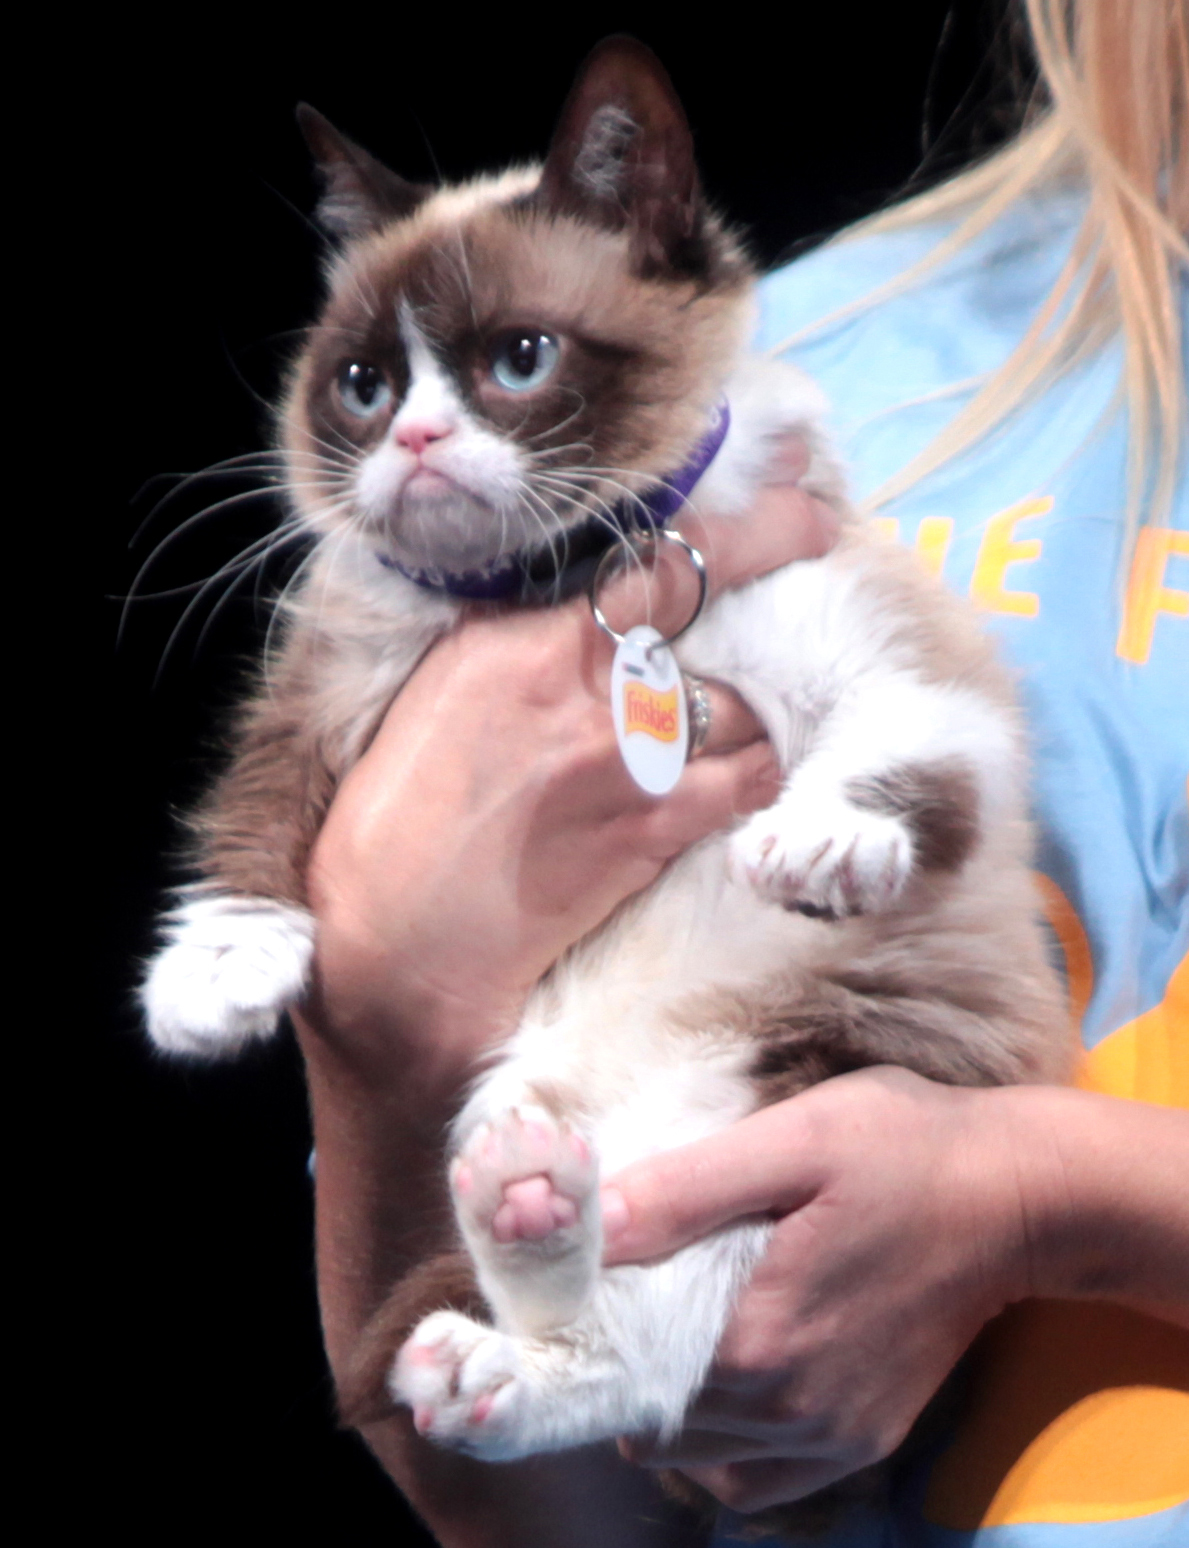
\includegraphics[width=50mm]{Grumpy_Cat_by_Gage_Skidmore.jpg}
\caption{Grumpy Cat}
\label{fig:Grumpy Cat}
\end{figure}

From figure \ref{fig:Grumpy Cat}, it is evident that the cat is grumpy.

\listoftables
\listoffigures
\end{document}